\chapter{Modelo Entidade Relacionamento}
 
O desenvolvimento de um Banco de Dados para uma aplicação, antes da implementação técnica, exige uma compreensão clara e estruturada dos dados que serão manipulados. Nesse contexto, o \textbf{Diagrama Entidade-Relacionamento (DER)} desempenha um papel fundamental no processo de modelagem de dados. O Diagrama Entidade-Relacionamento é um \textbf{modelo conceitual}, utilizado para representar, de forma abstrata e organizada, a estrutura das informações de um sistema. Ele está mais próximo da visão que o usuário possui dos dados, pois descreve os elementos do mundo real que serão armazenados e como eles se conectam entre si.

Por meio do DER, é possível identificar e definir:

\begin{itemize}
    \item Quais dados devem ser armazenados pela aplicação;
    \item As entidades que representam objetos ou conceitos do domínio do problema;
    \item Os atributos que caracterizam essas entidades;
    \item Como esses dados se relacionam entre si.
\end{itemize}

Dessa forma, o modelo Entidade-Relacionamento serve como base para a construção do modelo lógico e, posteriormente, do banco de dados físico. Ele contribui para reduzir ambiguidades, melhorar a comunicação entre desenvolvedores e usuários e garantir que o sistema atenda corretamente aos requisitos estabelecidos. Ao longo deste livro, serão apresentados os conceitos fundamentais do modelo Entidade-Relacionamento, suas notações, regras de construção e exemplos práticos, permitindo ao leitor compreender e aplicar essa importante ferramenta no projeto de bancos de dados. Abaixo está ilustrado um diagrama desse tipo:
\begin{diagramER}
\begin{center}
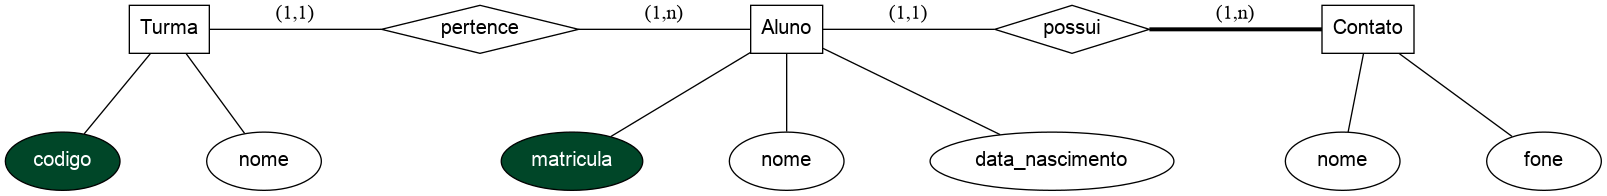
\includegraphics[width = 15.3cm]{er1.png}
\end{center}
\end{diagramER}

Antes de entendermos o diagrama, vejamos a Tabela~\ref{tab:elementos_der}. A Tabela~\ref{tab:elementos_der} apresenta os principais elementos que compõem o Diagrama Entidade-Relacionamento, destacando suas representações gráficas e respectivas funções no modelo conceitual. Os retângulos identificam os conjuntos de entidades, as elipses representam os atributos que descrevem suas características, os losangos indicam os relacionamentos estabelecidos entre entidades e as linhas evidenciam as conexões estruturais entre esses componentes. Em conjunto, esses elementos permitem a representação organizada e formal das informações de um domínio, servindo como base para a modelagem lógica e posterior implementação em banco de dados.


\begin{table}[h!]
\centering
\renewcommand{\arraystretch}{1.4}
\begin{tabular}{|p{3.5cm}|p{9cm}|}
\hline
\textbf{Elemento Gráfico} & \textbf{Descrição} \\ \hline

\textbf{Retângulo} &
Representa um \textit{conjunto de entidades}. Uma entidade corresponde a um objeto ou conceito do mundo real sobre o qual se deseja armazenar informações. Exemplos incluem \textit{Aluno}, \textit{Turma} ou \textit{Produto}. Cada instância da entidade possui existência própria dentro do sistema. \\ \hline

\textbf{Elipse} &
Representa um \textit{atributo}. Os atributos descrevem características ou propriedades das entidades ou dos relacionamentos. Exemplos incluem \textit{nome}, \textit{matrícula}, \textit{data\_nascimento}. Um atributo pode ser simples, composto, multivalorado ou chave. \\ \hline

\textbf{Losango} &
Representa um \textit{relacionamento}. O relacionamento descreve a associação existente entre dois ou mais conjuntos de entidades. Por exemplo, o relacionamento \textit{pertence} pode associar a entidade \textit{Aluno} à entidade \textit{Turma}. \\ \hline

\textbf{Linha} &
Representa a ligação entre elementos do diagrama. As linhas conectam atributos às entidades e entidades aos relacionamentos, indicando participação e associação estrutural no modelo conceitual. \\ \hline

\end{tabular}

\caption{Elementos fundamentais do Diagrama Entidade-Relacionamento}
\label{tab:elementos_der}

\end{table}
O Diagrama Entidade-Relacionamento apresentado modela um cenário acadêmico composto pelas entidades \textit{Turma}, \textit{Aluno} e \textit{Contato}. O modelo entidade-relacionamento tem por base a percepção de que o mundo real é formado por conjunto de objetos chamados entidades e pelo conjunto dos relacionamentos entre esses objetos. Retângulos, que representam os conjuntos de entidades; Elipses, que representam os atributos; Losangos, que representam os relacionamentos entre os conjuntos de entidades; Linhas, que unem os atributos aos conjuntos de entidades e o conjunto de entidades aos seus relacionamentos.

O modelo tem como objetivo representar a organização de alunos em turmas e o cadastro de contatos associados a cada aluno, evidenciando as estruturas de dados e as restrições de cardinalidade existentes no domínio analisado. A entidade \textbf{Turma} representa as unidades organizacionais às quais os alunos estão vinculados. Ela possui dois atributos: \textit{codigo}, que atua como chave primária e identifica unicamente cada turma no sistema, e \textit{nome}, que descreve a denominação da turma. A presença de uma chave primária garante a integridade da identificação das instâncias dessa entidade. A entidade \textbf{Aluno} representa os estudantes vinculados às turmas. Seus atributos são \textit{matricula}, \textit{nome} e \textit{data\_nascimento}. O atributo \textit{matricula} é definido como chave primária, sendo responsável por identificar de forma única cada aluno. Os demais atributos armazenam informações descritivas e complementares necessárias para caracterizar cada estudante.

A entidade \textbf{Contato} representa os dados de contato associados aos alunos. Ela possui os atributos \textit{nome} e \textit{fone}, que registram, respectivamente, o nome do contato e o número de telefone correspondente. Essa entidade permite armazenar múltiplos registros vinculados a um mesmo aluno. O relacionamento \textbf{pertence} estabelece a associação entre as entidades \textit{Aluno} e \textit{Turma}. A cardinalidade indicada no diagrama demonstra que cada aluno deve estar obrigatoriamente vinculado a exatamente uma turma, enquanto uma turma pode estar associada a um ou vários alunos. Trata-se, portanto, de um relacionamento do tipo um-para-muitos (1:N), com participação obrigatória do lado da entidade Aluno. O relacionamento \textbf{possui} associa a entidade \textit{Aluno} à entidade \textit{Contato}. A cardinalidade apresentada indica que cada aluno possui pelo menos um contato, podendo possuir vários, enquanto cada contato está vinculado a exatamente um aluno. Esse relacionamento também é classificado como um relacionamento do tipo um-para-muitos (1:N), com participação obrigatória da entidade Contato em relação ao aluno ao qual está associado.

De maneira geral, o modelo representa de forma consistente as restrições do domínio acadêmico considerado, garantindo identificação única das entidades principais e estabelecendo vínculos obrigatórios entre alunos e turmas, bem como entre alunos e seus respectivos contatos. A estrutura apresentada é adequada para posterior transformação em modelo relacional, preservando as chaves primárias e as dependências representadas pelas cardinalidades.

\section{Conceito de Atributos}

No modelo Entidade-Relacionamento, os \textbf{atributos} são as propriedades que descrevem as características de uma entidade ou de um relacionamento. Eles representam as informações que desejamos armazenar sobre cada ocorrência de uma entidade no sistema.

Cada entidade possui um conjunto próprio de atributos que definem seus dados. Por exemplo, a entidade \textbf{Professor} pode possuir atributos como matrícula, nome e telefone. A entidade \textbf{Disciplina} pode possuir atributos como código e nome. Já a entidade \textbf{Aluno} pode possuir atributos como matrícula, nome e data de nascimento.

\begin{figure}[h!]
    \centering
    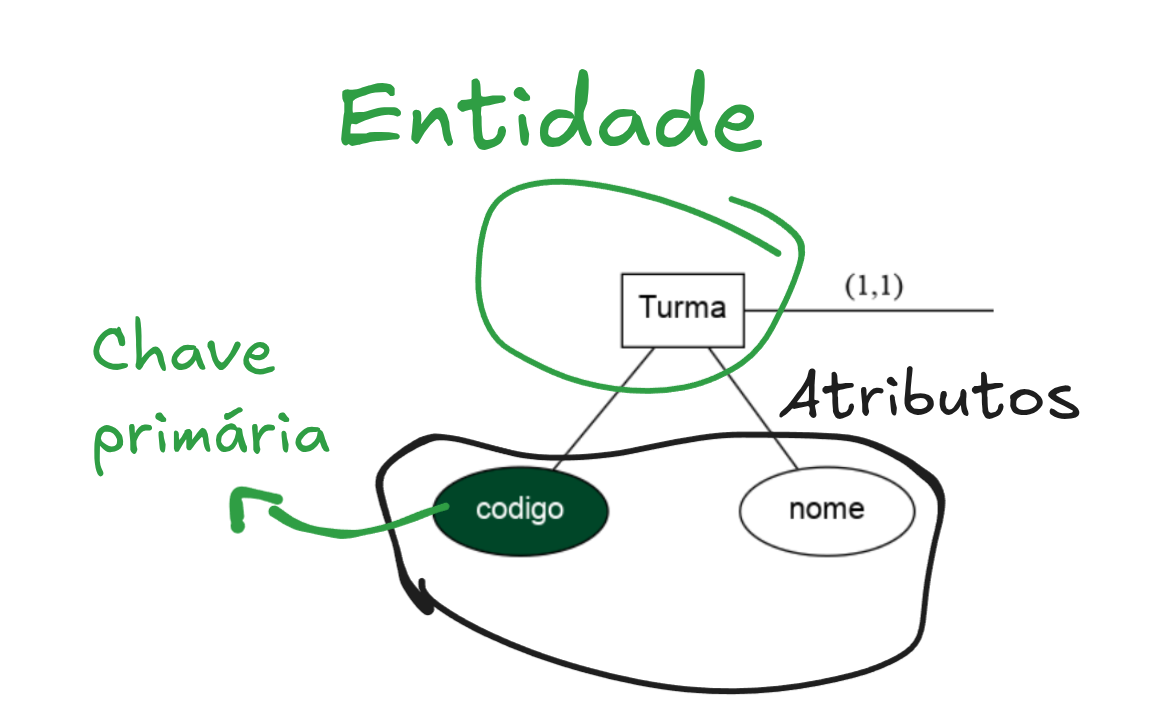
\includegraphics[width=15.3cm]{atributos.png}
    \caption{Atributos do Diagrama ER.}
    \label{fig:atributos}
\end{figure}




Os atributos podem ser classificados em diferentes tipos conceituais:

\begin{itemize}
    \item \textbf{Atributo simples}: não pode ser subdividido em partes menores (exemplo: matrícula).
    \item \textbf{Atributo composto}: pode ser dividido em subpartes (exemplo: um endereço poderia ser dividido em rua, número e cidade).
    \item \textbf{Atributo multivalorado}: pode assumir mais de um valor para a mesma entidade (exemplo: múltiplos telefones).
    \item \textbf{Atributo identificador (chave)}: atributo responsável por identificar unicamente cada ocorrência de uma entidade.
\end{itemize}

Os atributos são fundamentais para dar significado às entidades, pois sem eles não seria possível armazenar ou diferenciar as instâncias no banco de dados.

\section{Chave Primária}

Em um modelo de banco de dados relacional, a \textbf{chave primária} é o atributo, ou conjunto de atributos, responsável por identificar de maneira única cada registro de uma tabela. Isso significa que não podem existir duas linhas com o mesmo valor para a chave primária, garantindo que cada tupla seja distinta dentro da relação.

A principal função da chave primária é assegurar a integridade dos dados, evitando duplicidades e permitindo que cada registro seja referenciado de forma precisa. Para cumprir esse papel, ela deve apresentar algumas características fundamentais: seus valores devem ser únicos em toda a tabela, não podem assumir o valor \texttt{NULL}, devem ser preferencialmente estáveis ao longo do tempo (ou seja, não devem sofrer alterações frequentes) e devem conter apenas os atributos estritamente necessários para identificar o registro, preservando o princípio da minimalidade.

Como exemplo, considere a entidade \textit{Cliente}, composta pelos atributos id\_cliente, nome e telefone. Nesse caso, o atributo \texttt{id\_cliente} é definido como chave primária, pois identifica exclusivamente cada cliente no sistema, independentemente de possíveis repetições de nome ou telefone.

Em determinadas situações, a chave primária pode ser formada por mais de um atributo, caracterizando uma \textbf{chave primária composta}. Isso ocorre quando nenhum atributo isoladamente é capaz de garantir a identificação única do registro. Um exemplo comum é uma tabela que representa um relacionamento muitos-para-muitos entre as entidades \textit{Aluno} e \textit{Disciplina}. Nessa situação, a combinação dos atributos \texttt{id\_aluno} e \texttt{id\_disciplina} forma a chave primária, pois apenas o conjunto desses dois valores assegura a unicidade de cada registro.

Assim, a definição adequada da chave primária é essencial no modelo relacional, pois possibilita o estabelecimento correto de relacionamentos entre tabelas, previne inconsistências e mantém a integridade referencial do banco de dados. Por esse motivo, toda tabela deve possuir uma chave primária claramente definida.

\section{Conceito de Relacionamentos}

Os \textbf{relacionamentos} representam as associações existentes entre duas ou mais entidades dentro do modelo. Eles indicam como as entidades se conectam e interagem no domínio do problema. Um relacionamento pode ser classificado de acordo com sua \textbf{cardinalidade}, que define o número mínimo e máximo de ocorrências de uma entidade que podem estar associadas a outra. As cardinalidades mais comuns são:

\begin{itemize}
    \item \textbf{Um-para-um (1:1)}: uma ocorrência de uma entidade está associada a apenas uma ocorrência da outra.
    \item \textbf{Um-para-muitos (1:N)}: uma ocorrência de uma entidade pode estar associada a várias ocorrências da outra.
    \item \textbf{Muitos-para-muitos (N:M)}: várias ocorrências de uma entidade podem estar associadas a várias ocorrências da outra.
\end{itemize}

\begin{diagramER}
\begin{center}
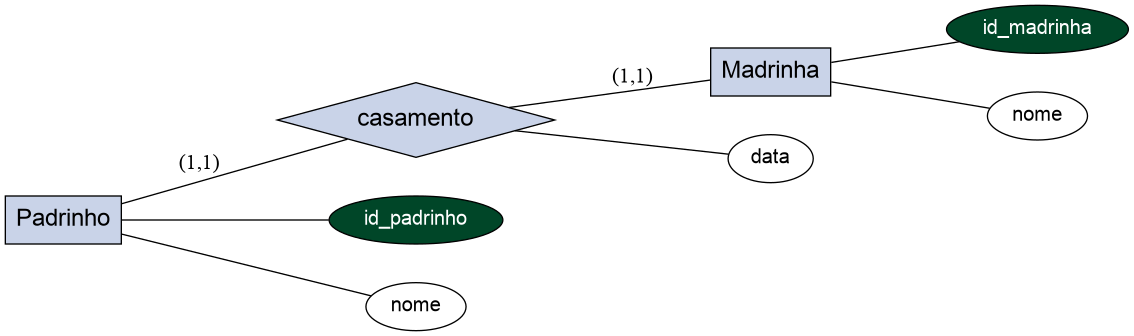
\includegraphics[width = 15.3cm]{er_1_1.png}
\end{center}
\end{diagramER}\begin{observacao}
No primeiro diagrama, é apresentado um relacionamento do tipo um-para-um (1:1) entre as entidades Padrinho e Madrinha, mediado pelo relacionamento casamento. A cardinalidade (1,1) em ambos os lados indica que cada padrinho está associado a exatamente uma madrinha, e cada madrinha está associada a exatamente um padrinho dentro do contexto modelado. Isso caracteriza uma associação exclusiva entre as duas entidades. Cada entidade possui um atributo identificador destacado como chave primária id\_padrinho e id\_madrinha, cuja função é garantir a identificação única de cada ocorrência. Além disso, ambas possuem atributos descritivos, como nome. O relacionamento casamento também possui um atributo próprio, data, que armazena uma informação específica da associação entre padrinho e madrinha, demonstrando que relacionamentos também podem possuir atributos quando é necessário registrar características do vínculo entre as entidades.
\end{observacao}
\begin{diagramER}
\begin{center}
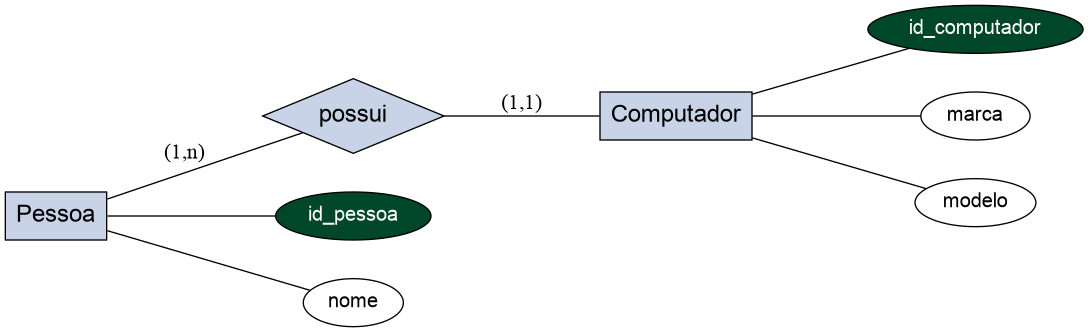
\includegraphics[width = 15.3cm]{er_1_n.png}
\end{center}
\end{diagramER}\begin{observacao}
No segundo diagrama, é representado um relacionamento do tipo um-para-muitos (1:N) entre as entidades Pessoa e Computador, por meio do relacionamento possui. A cardinalidade (1,n) do lado de Pessoa indica que uma pessoa pode possuir vários computadores, enquanto a cardinalidade (1,1) do lado de Computador indica que cada computador pertence a exatamente uma pessoa. Esse tipo de modelagem é comum quando um elemento principal pode estar associado a várias ocorrências de outro elemento dependente. A entidade Pessoa possui como chave primária o atributo id\_pessoa, além do atributo descritivo nome. A entidade Computador possui id\_computador como chave primária, além dos atributos marca e modelo. Neste caso, o relacionamento não possui atributos próprios, pois a associação “possui” não necessita armazenar informações adicionais além da ligação entre as entidades.
\end{observacao}

\begin{diagramER}
\begin{center}
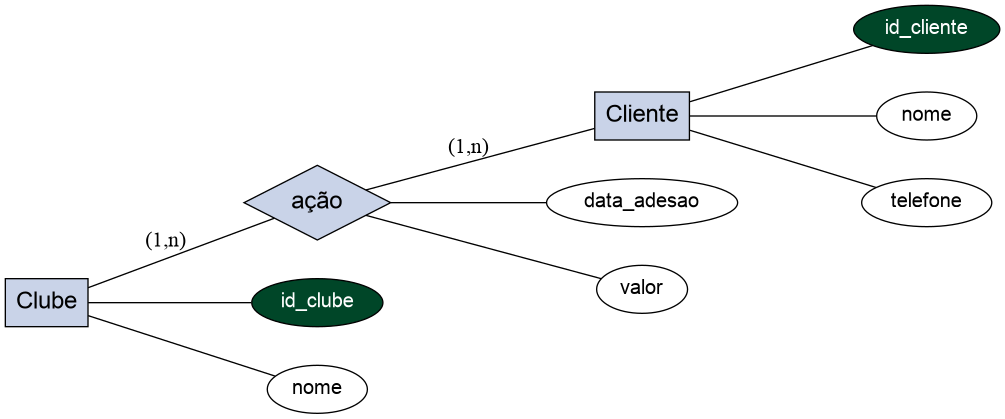
\includegraphics[width = 15.3cm]{er_n_n_.png}
\end{center}
\end{diagramER}
\begin{observacao}
No terceiro diagrama, é apresentado um relacionamento do tipo muitos-para-muitos (N:M) entre as entidades Clube e Cliente, por meio do relacionamento ação. A cardinalidade \(1,n\) em ambos os lados indica que um clube pode estar associado a vários clientes e que um cliente pode participar de vários clubes simultaneamente. Esse tipo de relacionamento representa uma associação múltipla em ambas as direções, sendo bastante comum em sistemas reais. 

A entidade Clube possui id\_clube como chave primária e nome como atributo descritivo, enquanto a entidade Cliente possui id\_cliente como chave primária, além de nome e telefone. Diferentemente do caso anterior, o relacionamento ação possui atributos próprios, como data\_adesao e valor, que armazenam informações específicas da participação do cliente no clube. 

Isso demonstra que, em relacionamentos muitos-para-muitos, é frequente a necessidade de registrar dados adicionais referentes à própria associação.
\end{observacao}

Além disso, os relacionamentos podem possuir atributos próprios, quando é necessário armazenar informações específicas sobre a associação entre as entidades. Portanto, enquanto as entidades representam os objetos principais do domínio e os atributos descrevem suas características, os relacionamentos estabelecem as ligações estruturais que organizam o modelo de dados.

\section{Exemplo de diagrama ER}
  O diagrama Entidade-Relacionamento apresentado é composto por três entidades principais: \textbf{Professor}, \textbf{Disciplina} e \textbf{Aluno}. Essas entidades representam os objetos fundamentais do domínio acadêmico modelado. A entidade \textbf{Professor} representa os docentes responsáveis pela oferta das disciplinas. Já a entidade \textbf{Disciplina} representa as matérias ofertadas na instituição. Por sua vez, a entidade \textbf{Aluno} representa os estudantes matriculados na instituição. Entre essas entidades existem dois relacionamentos principais. O primeiro relacionamento, denominado \textbf{leciona}, conecta as entidades \textbf{Professor} e \textbf{Disciplina}. A cardinalidade indica que cada professor participa do relacionamento com cardinalidade (1,1), enquanto cada disciplina participa com cardinalidade (1,n). Isso significa que um professor está associado a exatamente uma ocorrência no relacionamento, enquanto uma disciplina pode estar associada a uma ou várias ocorrências conforme definido no modelo. O segundo relacionamento, denominado \textbf{estuda}, conecta as entidades \textbf{Disciplina} e \textbf{Aluno}. A cardinalidade (1,n) em ambos os lados indica que uma disciplina pode estar relacionada a vários alunos e que um aluno pode estar relacionado a várias disciplinas, caracterizando um relacionamento do tipo muitos-para-muitos.

Assim, o modelo descreve a estrutura básica de um sistema acadêmico no qual professores lecionam disciplinas e alunos estudam disciplinas, estabelecendo as ligações essenciais entre os principais elementos do domínio. 

\begin{diagramER}
\begin{center}
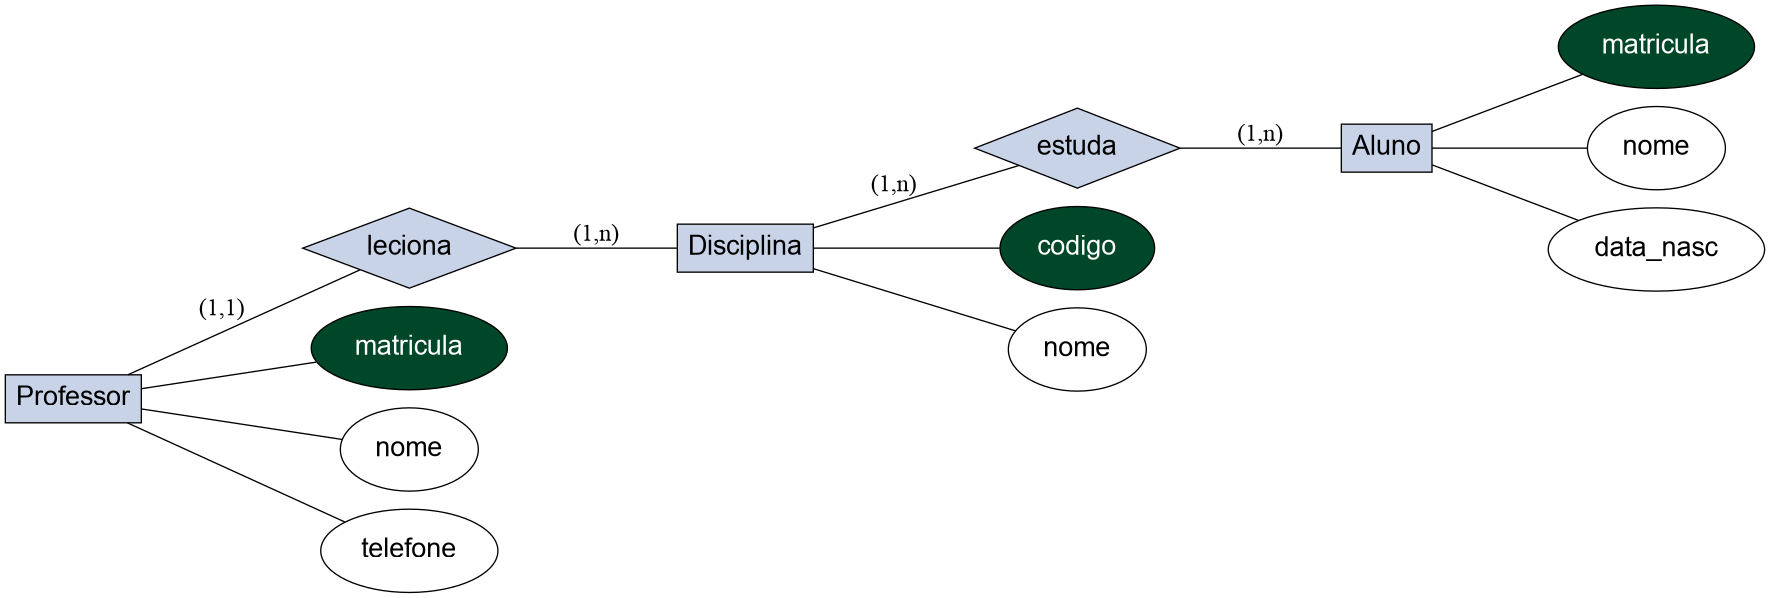
\includegraphics[width = 15.3cm]{er2.png}
\end{center}
\end{diagramER}

\section{Atividade prática de MER}

\subsection{Objetivo}
O objetivo desta atividade é desenvolver a capacidade de análise de requisitos e modelagem conceitual de um banco de dados por meio da construção de um \textbf{Diagrama Entidade-Relacionamento (DER)} para um sistema realista de controle de ordenha em uma fazenda leiteira.

\subsection{Contexto do Sistema}

\begin{center}
    
\includegraphics[width=9cm]{fazenda.png}
    \captionof{figure}{Uma fazenda da cidade de Rio Verde. Fonte: Instagram @fazendanycolle}
\end{center}

Uma fazenda leiteira deseja informatizar o controle de suas atividades de ordenha. Atualmente, os registros são feitos manualmente, o que dificulta o acompanhamento da produção, da saúde dos animais e do desempenho dos funcionários. O sistema deverá armazenar informações sobre as vacas, as ordenhas realizadas, os funcionários responsáveis, os equipamentos utilizados e a produção de leite obtida em cada ordenha.

\subsection{Descrição dos Requisitos}

Abaixo são detalhados os requisitos levantados para a modelagem do sistema:

\subsubsection{Vacas}
Cada vaca da fazenda deve ser identificada por um código único. Além disso, devem ser armazenadas informações como:
\begin{itemize}
    \item Nome ou identificação visual;
    \item Data de nascimento;
    \item Raça, Peso e Status de saúde.
\end{itemize}

\subsubsection{Funcionários e Supervisão}
A fazenda possui funcionários com diferentes atribuições:
\begin{itemize}
    \item \textbf{Funcionários de Campo:} Registrados por código, nome completo, função (ordenhador, etc.) e telefone.
    \item \textbf{Supervisor:} Responsável por acompanhar o trabalho. Registra-se código, nome, telefone e turno de supervisão.
    \item \textbf{Veterinário:} Responsável pela saúde clínica. Registra-se código, nome, registro profissional (CRMV) e telefone.
\end{itemize}

\subsubsection{Processo de Ordenha}
A ordenha ocorre diariamente e pode acontecer mais de uma vez por dia para a mesma vaca. Cada registro de ordenha deve conter: \textbf{Data, Horário e Quantidade de leite (litros)}.

\subsection{Regras de Negócio e Relacionamentos}

Para facilitar o entendimento das cardinalidades, o produtor descreveu a rotina da seguinte forma:

\begin{block}{Rotina de Ordenha}
Cada vaca da fazenda é ordenhada ao longo do tempo. Em alguns períodos, a mesma vaca pode ser ordenhada mais de uma vez no mesmo dia. Sempre que ocorre uma ordenha, ela diz respeito a uma única vaca.
\end{block}

\begin{block}{Trabalho dos Funcionários}
Os funcionários são responsáveis por realizar as ordenhas. Um mesmo funcionário pode ordenhar várias vacas ao longo do dia. No entanto, toda ordenha precisa ter alguém responsável por realizá-la.
\end{block}

\begin{block}{Uso dos Equipamentos}
Para realizar a ordenha, podem ser usados um ou vários equipamentos (manuais, automáticos ou robóticos). Os equipamentos podem ser utilizados em diferentes ordenhas ou ficar parados para manutenção.
\end{block}

\begin{block}{Cuidado com a Saúde}
O veterinário pode atender várias vacas ao longo do tempo e, dependendo do caso, a mesma vaca pode precisar de mais de um atendimento em momentos diferentes.
\end{block}

\begin{block}{Visão do Proprietário}
O proprietário não participa da ordenha diretamente, mas acompanha os relatórios de produção, desempenho da equipe e utilização de equipamentos para tomada de decisão.
\end{block}

\subsection{Atividades Propostas}

Com base na descrição acima, realize a modelagem conceitual seguindo os passos:
\begin{enumerate}
    \item Identifique todas as \textbf{entidades} do sistema.
    \item Para cada entidade, defina seus \textbf{atributos} e a \textbf{chave primária}.
    \item Modele os \textbf{relacionamentos} (ex: Vaca \textit{sofre} Ordenha).
    \item Defina as \textbf{cardinalidades} (1:1, 1:N, N:M) e a \textbf{participação} (total ou parcial).
    \item Identifique se há necessidade de atributos nos relacionamentos.
\end{enumerate}

\begin{observacao}
\textbf{Instruções de Entrega:}
O Diagrama Entidade-Relacionamento deve ser feito de forma legível (à mão ou ferramenta digital como brModelo/Lucidchart). O arquivo final deve ser convertido para \textbf{PDF} e conter apenas o diagrama finalizado.
\end{observacao}

\subsection{Critérios de Avaliação}
A avaliação considerará a correta identificação das entidades, adequação das chaves primárias, precisão das cardinalidades frente às regras de negócio e a organização visual do diagrama.

\vspace{0.5cm}
